% Contenidos del capítulo.
% Las secciones presentadas son orientativas y no representan
% necesariamente la organización que debe tener este capítulo.

% Introducción
En el presente capítulo se lleva a cabo un análisis del estado del arte con el fin de situar el 
proyecto en el contexto de soluciones existentes y tecnologías actuales. La plataforma 
web desarrollada en este \gls{tfg} tiene como objetivo facilitar el emparejamiento entre 
profesionales y proyectos mediante un sistema basado en competencias jerarquizadas. 
Por ello, resulta esencial estudiar qué herramientas similares existen ya en el mercado 
y cómo se enfrentan a problemas de emparejamiento, recomendación o gestión de 
talento y proyectos.

Primero se presentarán aplicaciones con funcionalidades relacionadas, analizando sus 
características principales, puntos en común con esta propuesta y diferencias clave. 
Este estudio permitirá identificar tanto aspectos que se consideran imprescindibles en 
una plataforma de este tipo, como oportunidades de mejora o innovación.

Posteriormente se realizará un análisis crítico de las tecnologías más relevantes para el 
desarrollo del sistema, justificando la elección final en cada caso a partir de criterios 
como la escalabilidad, facilidad de desarrollo, mantenimiento o compatibilidad entre 
componentes.

Por último, se listarán aquellas herramientas de soporte utilizadas durante el desarrollo 
del \gls{tfg}, como entornos de desarrollo, sistemas de control de versiones o editores 
de diagramas, las cuales han sido fundamentales para llevar a cabo el proyecto.

% 2.1
\section{Análisis de aplicaciones similares}
% Qué aplicaciones similares hay y en qué se diferencia de ellas la propuesta
En esta sección se analizarán distintas aplicaciones existentes que presentan elementos 
comunes con la \textbf{plataforma web desarrollada en este trabajo}, cuyo objetivo es 
facilitar el \textbf{emparejamiento entre profesionales y proyectos} en función de sus 
competencias. Para ello, se comentarán \textbf{soluciones reales} que abordan problemas 
similares, ya sea desde la perspectiva de \textbf{plataformas orientadas al empleo y el talento}, 
o desde el enfoque de \textbf{sistemas de emparejamiento inteligente basados en afinidad}.

Dado que el proyecto combina ideas presentes en entornos profesionales como LinkedIn \cite{linkedin}
y en algoritmos de emparejamiento como los utilizados por aplicaciones tipo Tinder \cite{tinder}, se 
ha optado por dividir este análisis en \textbf{dos bloques diferenciados}. En el primero se 
estudiarán \textbf{plataformas centradas en la gestión del talento y la búsqueda de empleo}, 
mientras que en el segundo se abordarán \textbf{sistemas cuyo núcleo es el emparejamiento 
basado en coincidencias}, con el objetivo de extraer ideas aplicables al 
\gls{recomendaciones} que se desea implementar.

Este análisis permitirá no solo \textbf{identificar funcionalidades clave y enfoques existentes}, 
sino también detectar \textbf{carencias o posibles áreas de mejora}, con el fin de proponer 
una solución más \textbf{adaptada, automatizada} y centrada en la 
\textbf{coincidencia de competencias concretas}.

% 2.1.1
\subsection{Plataformas web orientadas al empleo y la gestión del talento}

Dado que la plataforma web a desarrollar tiene como objetivo conectar profesionales con 
proyectos en función de sus competencias, las primeras aplicaciones a analizar son aquellas 
centradas en la búsqueda de empleo, la exposición del perfil profesional y la gestión del talento.

En esta sección se analizarán concretamente las plataformas \textbf{LinkedIn} \cite{linkedin}, 
\textbf{InfoJobs} \cite{infojobs} y \textbf{Yobalia} \cite{yobalia}, destacando sus funcionalidades principales y su grado 
de similitud con la solución propuesta en este trabajo.

% LinkedIn
\subsubsection{LinkedIn}

En primer lugar, \textbf{LinkedIn} \cite{linkedin} es una plataforma web orientada al entorno 
profesional que permite a los usuarios crear un perfil con información detallada sobre su 
experiencia laboral, formación académica, certificaciones y competencias. Su objetivo 
principal es facilitar la conexión entre profesionales, empresas y oportunidades laborales, 
actuando como red social y como herramienta para la búsqueda de empleo.

Entre sus funcionalidades destaca un sistema de filtrado de ofertas que permite ajustar la 
búsqueda según múltiples parámetros, como ubicación, modalidad de trabajo (presencial o 
remoto), tipo de contrato o experiencia requerida. En la Figura \ref{fig:linkedin-ofertas} se muestra un ejemplo de 
búsqueda activa de empleo, donde se visualizan las ofertas disponibles y una vista previa de 
cada una de ellas. En particular, se ha realizado una búsqueda real orientada al perfil de 
\textbf{programador \gls{fullstack}} en la zona de \textbf{Valencia}, comprobando que la 
plataforma devuelve resultados actualizados y relevantes. Esta funcionalidad se basa en un 
sistema de filtrado tradicional implementado sobre formularios dinámicos en el 
\gls{frontend}, que construyen consultas específicas para recuperar ofertas desde su 
\gls{backend}.

Además, LinkedIn ofrece la posibilidad de añadir \textit{habilidades} al perfil de usuario, 
las cuales pueden ser validadas por otros contactos, y que posteriormente pueden ser 
utilizadas por los reclutadores para filtrar candidatos en función de sus aptitudes. 
En la Figura \ref{fig:linkedin-aptitudes} se ilustra esta sección del perfil. A pesar de ello, la plataforma no 
implementa un sistema de recomendaciones basado en coincidencias automáticas entre 
el perfil y las ofertas, sino que es el propio usuario quien debe llevar a cabo la búsqueda 
activa.

LinkedIn también dispone de herramientas de suscripción premium, que permiten acceder a 
estadísticas avanzadas sobre las postulaciones o enviar mensajes directos a reclutadores. 
Sin embargo, para el uso básico, la mayoría de funcionalidades son gratuitas.

En definitiva, LinkedIn representa un referente consolidado en la búsqueda de empleo y la 
gestión del talento, pero su funcionamiento está centrado en la exploración manual y el 
uso de filtros, sin un sistema automatizado de emparejamiento como el que se plantea en 
este trabajo.

\begin{figure}[H]
    \centering
    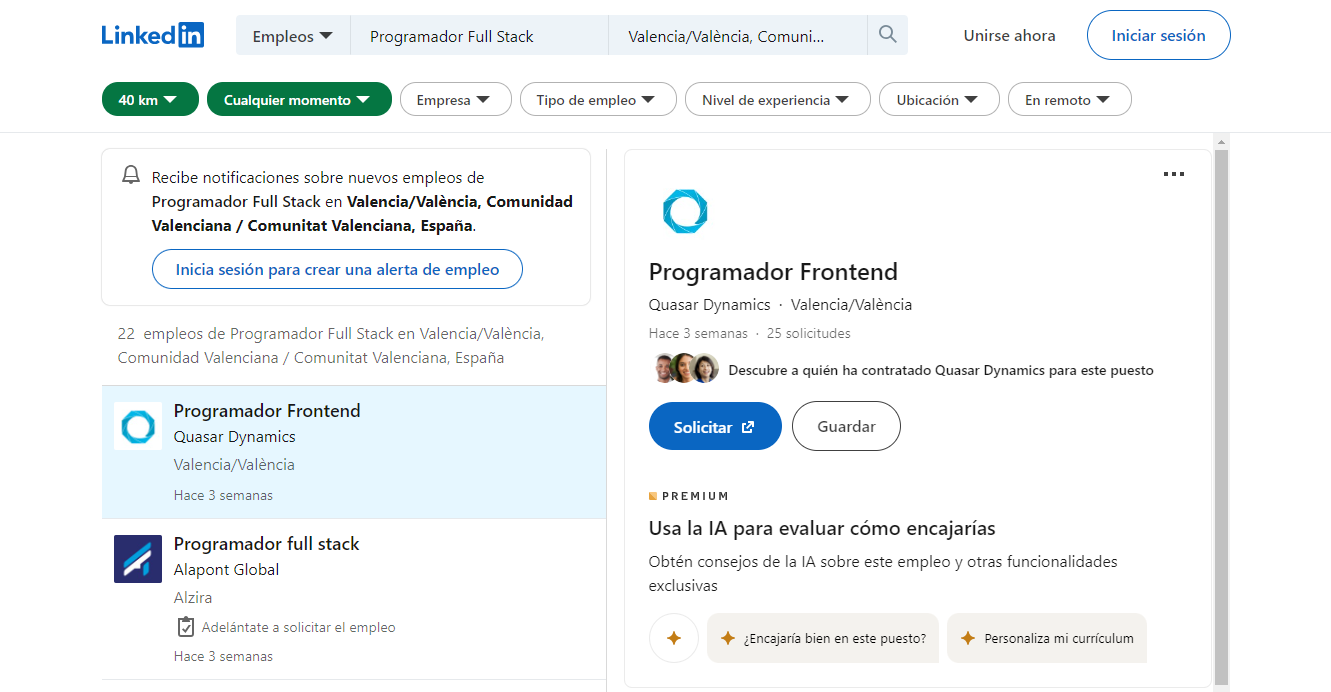
\includegraphics[width=0.9\textwidth]{figs/linkedin-ofertas.png}
    \caption{Interfaz de búsqueda de empleo en LinkedIn para ``Programador Full Stack''.}
    \label{fig:linkedin-ofertas}
  \end{figure}
  
\begin{figure}[H]
    \centering
    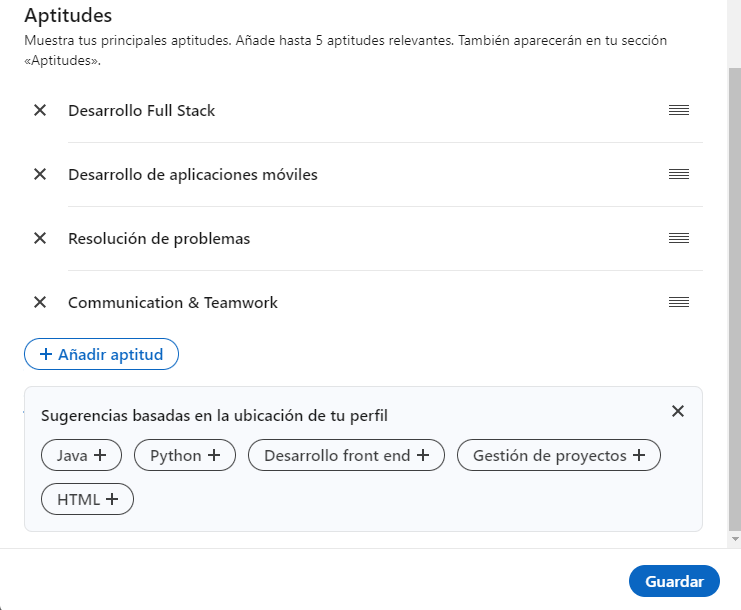
\includegraphics[width=0.65\textwidth]{figs/linkedin-aptitudes.png}
    \caption{Ejemplo de selección de aptitudes en el perfil de usuario de LinkedIn.}
    \label{fig:linkedin-aptitudes}
\end{figure}

% InfoJobs
\subsubsection{InfoJobs}

\textbf{InfoJobs} \cite{infojobs} es una plataforma generalista de búsqueda de empleo en España, 
orientada a la publicación y gestión de ofertas laborales de múltiples sectores. A diferencia de 
\textbf{LinkedIn}, su funcionamiento se centra en la inscripción directa del usuario a las ofertas, sin 
red de contactos ni validación de aptitudes.

Este sistema de búsqueda utiliza formularios predefinidos en el frontend para generar filtros 
que se aplican sobre la base de datos mediante consultas directas al backend, priorizando 
coincidencias exactas entre los criterios seleccionados y los campos del perfil del usuario. 
Sin embargo, no emplea ningún tipo de lógica avanzada de emparejamiento automático o inferencia 
basada en competencias.

En la Figura~\ref{fig:infojobs-oferta} se muestra un ejemplo de oferta publicada para un puesto de 
programador web, donde se observan los detalles del puesto, los requisitos y las opciones de inscripción.

Frente a este enfoque, la plataforma propuesta en este \gls{tfg} plantea un sistema de recomendaciones 
que busca automatizar el emparejamiento, priorizando aquellas coincidencias más relevantes entre 
las competencias del profesional y las necesidades del proyecto.

\begin{figure}[H]
    \centering
    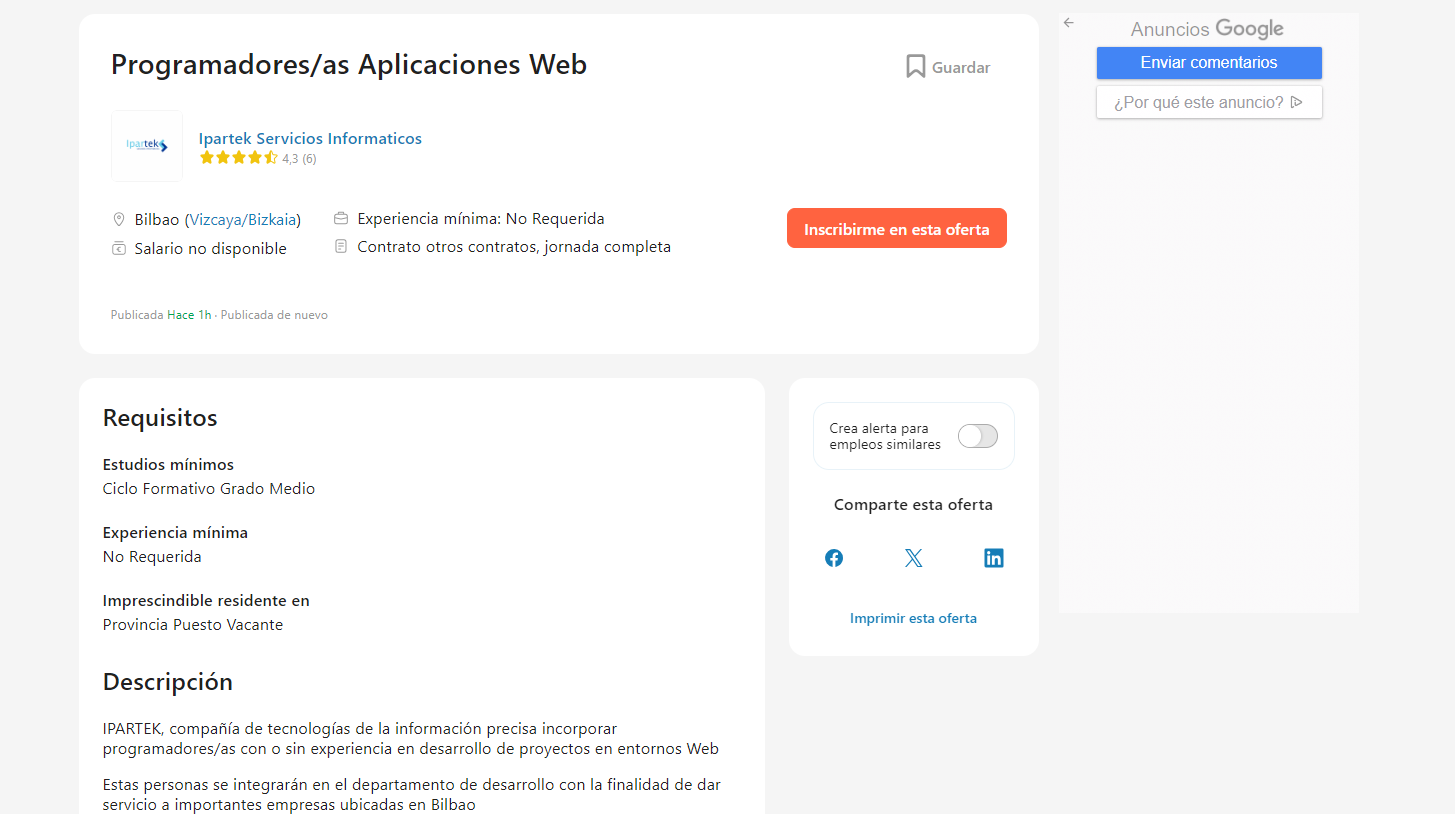
\includegraphics[width=0.85\textwidth]{figs/infojobs-oferta.png}
    \caption{Ejemplo de oferta de trabajo publicada en InfoJobs.}
    \label{fig:infojobs-oferta}
\end{figure}

% Yobalia
\subsubsection{Yobalia}

Por último, \textbf{Yobalia} \cite{yobalia} es una plataforma web de búsqueda de empleo especializada en 
el sector de eventos, promociones y acciones publicitarias. Está orientada principalmente a perfiles como 
azafatas, promotores, animadores o personal para campañas de marketing en punto de venta.

Desde su página principal queda patente esta orientación, posicionándose como un portal de referencia 
para trabajos puntuales y de corta duración. En la Figura \ref{fig:yobalia-portada} se muestra su interfaz 
de búsqueda, donde es posible filtrar las ofertas disponibles mediante criterios básicos como la ubicación, 
la categoría profesional o palabras clave introducidas por el usuario. Este último elemento guarda cierta 
relación con el sistema basado en competencias que plantea la solución de este \gls{tfg}, si bien su 
funcionamiento se basa en una coincidencia textual directa sin ningún tipo de análisis semántico o ponderación.

Aunque permite registrar el currículum y aplicar de forma rápida a las ofertas, la plataforma carece de 
validación de habilidades, conexión entre perfiles o mecanismos automatizados de emparejamiento. Todo el 
proceso de búsqueda y postulación depende de la acción manual del usuario.

En este sentido, la plataforma propuesta en este trabajo no solo abarca perfiles técnicos, sino que también 
está concebida para facilitar el acceso a trabajos eventuales como los ofrecidos en Yobalia, mejorando la 
eficiencia del proceso mediante un sistema de recomendaciones que prioriza las coincidencias entre requisitos 
y competencias de forma más automatizada.

\begin{figure}[H]
    \centering
    
\includegraphics[width=0.85\textwidth]{figs/yobalia-portada.png}
    \caption{Interfaz principal de búsqueda de empleo en Yobalia, con filtros por ubicación, categoría y palabras clave.}
    \label{fig:yobalia-portada}
\end{figure}

% Conclusiones sobre plataformas orientadas al empleo
\subsubsection{Conclusiones}

Tras analizar las plataformas presentadas, podría cuestionarse si hubiera sido más
eficiente utilizar directamente alguna de ellas para gestionar el emparejamiento entre
profesionales y proyectos. Sin embargo, existen motivos claros para optar por una
\textbf{plataforma desarrollada a medida}.

\textbf{LinkedIn}, aunque potente, es una red generalista donde el emparejamiento entre
usuarios y ofertas no se basa en un \textbf{sistema automático guiado por competencias},
sino en la búsqueda activa y manual. \textbf{InfoJobs}, por su parte, se basa en filtros
simples definidos por las ofertas, sin aplicar lógica de emparejamiento basada en
competencias reales. Finalmente, \textbf{Yobalia} está centrada en trabajos puntuales y
carece de un \textbf{sistema de recomendación avanzado}.

Por tanto, desarrollar una solución propia permite construir un modelo \textbf{centrado en
competencias}, adaptable a distintos tipos de perfiles y proyectos, y con capacidad de
evolución. Esta decisión garantiza una mayor \textbf{flexibilidad} y un \textbf{control
total} sobre la funcionalidad y el enfoque del sistema, ajustándose plenamente a los
objetivos de este \gls{tfg}.

% 2.1.2
\subsection{Aplicaciones con sistemas de emparejamiento basados en coincidencias}

Una vez analizadas las plataformas orientadas al empleo y la gestión del talento, es
interesante estudiar ciertas aplicaciones que, aunque no estén diseñadas con un fin
profesional, hacen uso de sistemas de emparejamiento o recomendación basados en la
coincidencia entre perfiles, intereses o preferencias. Estas soluciones ofrecen ideas
relevantes que pueden ser adaptadas a un contexto donde las competencias técnicas son el
eje central del emparejamiento.

En este apartado se analizarán tres casos representativos. En primer lugar, \textbf{Tinder} \cite{tinder},
como referente en emparejamiento entre personas a través de la coincidencia de interés
mutuo. A continuación, \textbf{Spotify} \cite{spotify}, cuyo sistema de recomendaciones personalizadas
brinda conceptos aplicables (sin entrar en la complejidad de sus algoritmos internos). Por
último, \textbf{Shapr} \cite{shapr}, que traslada la lógica de afinidad al entorno profesional,
sugiriendo perfiles compatibles según objetivos e intereses compartidos.

El objetivo es extraer elementos útiles como la personalización, la afinidad o la lógica
de coincidencia, con el fin de incorporarlos a un sistema más estructurado y adaptado al
emparejamiento entre profesionales y proyectos según sus competencias.

% Tinder
\subsubsection{Tinder}

\textbf{Tinder} \cite{tinder} es una aplicación centrada en el emparejamiento entre
personas mediante la coincidencia de intereses. El sistema sugiere perfiles según criterios
como edad, género y ubicación, y cada usuario decide si le interesa o no. Cuando ambas
personas muestran interés, se genera un \gls{match} que permite iniciar una conversación.

Parte de la lógica que sigue Tinder está basada en los gustos personales, que pueden indicarse al
crear el perfil, como se muestra en la Figura \ref{fig:tinder-intereses}. Sin embargo, esta
información es completamente opcional y no condiciona el funcionamiento del sistema, que se
basa principalmente en la acción voluntaria del usuario, recogiendo principalmente otros
parámetros obligatorios como la ubicación, edad, tipo de relación, etc.

La plataforma propuesta en este trabajo recoge esa idea de emparejar por afinidad, pero la
lleva a un terreno más técnico. En lugar de basarse únicamente en preferencias generales o
gustos personales, los profesionales deben definir competencias concretas mediante palabras
clave, además de otros datos como la ubicación o el tipo de proyecto deseado. A diferencia
de Tinder, donde el emparejamiento depende de la acción mutua de los usuarios, aquí se
realiza de forma automática en función del grado de coincidencia entre los perfiles y los
requisitos definidos, permitiendo una búsqueda más eficiente y adaptada a las necesidades de
cada usuario.

\begin{figure}[H]
    \centering
    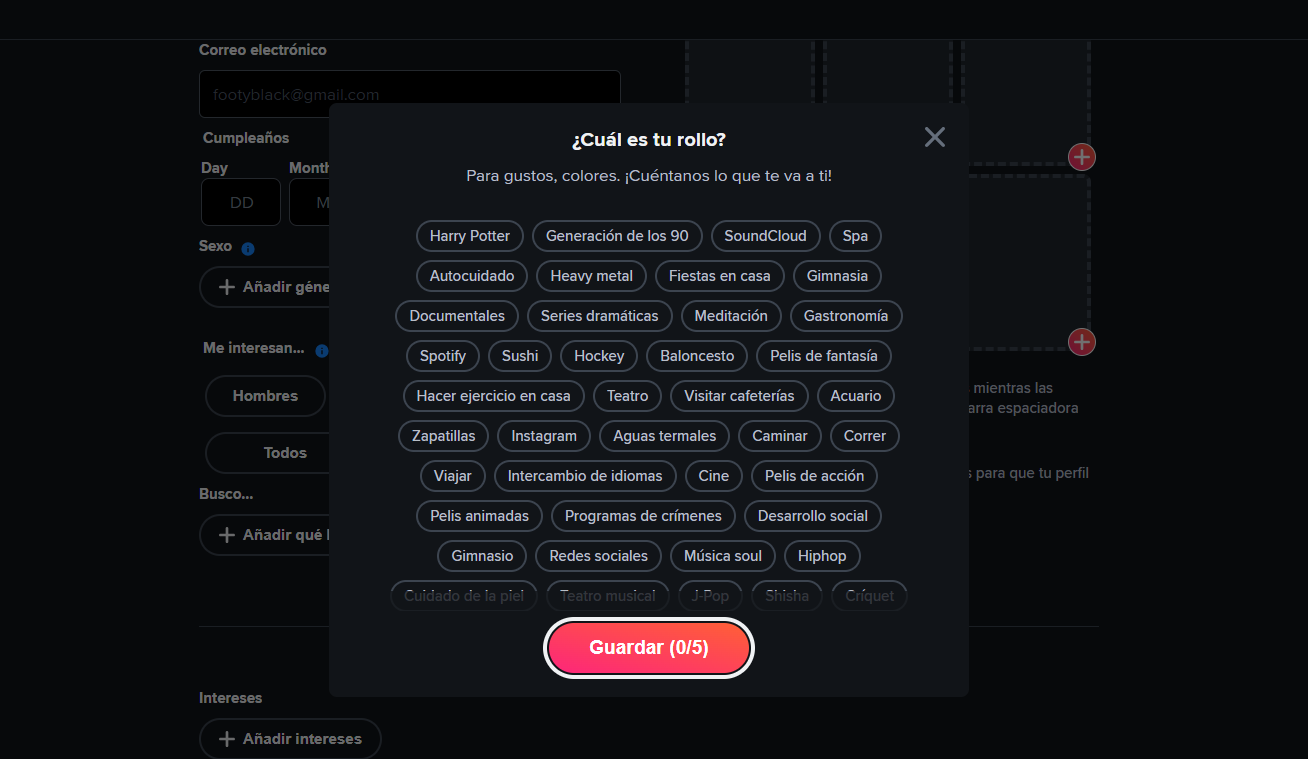
\includegraphics[width=0.85\textwidth]{figs/tinder-intereses.png}
    \caption{Selección opcional de intereses en Tinder durante la creación del perfil.}
    \label{fig:tinder-intereses}
\end{figure}

% Spotify
\subsubsection{Spotify}

\textbf{Spotify} \cite{spotify} es una plataforma de música en streaming que destaca por
su sistema de recomendaciones personalizadas. A partir del historial de escucha, listas
guardadas o canciones favoritas, sugiere contenido ajustado a los gustos del usuario.

En la Figura \ref{fig:spotify-mixes} se muestran ejemplos de \textit{Mixes diarios},
listas generadas automáticamente en función de preferencias individuales. De forma
similar, la Figura \ref{fig:spotify-videos} muestra una selección de vídeos musicales
relevantes para el perfil del usuario.

Aunque Spotify no empareja personas, su modelo sirve de referencia para esta plataforma,
especialmente en dos aspectos: mostrar resultados filtrados y relevantes en lugar de
listados genéricos, y calcular una \textbf{afinidad cuantificada} entre usuarios y
contenido, concepto que se traslada aquí al emparejamiento entre profesionales y proyectos.

\begin{figure}[H]
    \centering
    
\includegraphics[width=0.9\textwidth]{figs/spotify-mixes.png}
    \caption{Recomendaciones musicales personalizadas mediante mezclas diarias en Spotify.}
    \label{fig:spotify-mixes}
\end{figure}

\begin{figure}[H]
    \centering
    
\includegraphics[width=0.9\textwidth]{figs/spotify-videos.png}
    \caption{Selección de vídeos musicales adaptados a los gustos del usuario.}
    \label{fig:spotify-videos}
\end{figure}

% Shapr
\subsubsection{Shapr}

\textbf{Shapr} \cite{shapr} es una aplicación de networking profesional que emplea un
sistema de emparejamiento entre usuarios a partir de información como el área profesional,
ubicación, experiencia, año académico e intereses generales. A diario sugiere un número
limitado de perfiles o empleos potencialmente afines, ofreciendo una experiencia sencilla
y enfocada en generar conexiones útiles.

Aunque está centrada en el ámbito profesional, Shapr no funciona como un portal de empleo
tradicional, sino que utiliza una lógica de emparejamiento basada en sugerencias
automatizadas y validación mutua, similar a lo que ocurre en aplicaciones como Tinder. Por
este motivo, se ha incluido en este bloque, centrado en sistemas de coincidencia, y no en
el anterior, dedicado a plataformas orientadas a la gestión del talento.

En la Figura \ref{fig:shapr-ofertas} se muestra su sección de ofertas laborales, donde se
presentan prácticas o puestos adaptados al perfil del usuario. Este filtrado no requiere
una búsqueda activa ni ajustes manuales por parte del usuario, como sucede en plataformas
como LinkedIn. En su lugar, el sistema interpreta automáticamente los datos proporcionados,
como el grado, la ubicación o el año académico. Por ejemplo, si el usuario indica que está
cursando el último año de carrera, es habitual que se prioricen ofertas de prácticas o
contratos de formación.

A diferencia de las plataformas anteriores, Shapr sí está enfocada al entorno profesional,
lo que la convierte en una referencia especialmente relevante para este trabajo. La
plataforma propuesta recoge esa misma idea de sencillez en la presentación, pero la aplica
al sistema ya comentado, basado en competencias y coincidencias automáticas, acompañado de
un indicador de afinidad.

\begin{figure}[H]
    \centering
    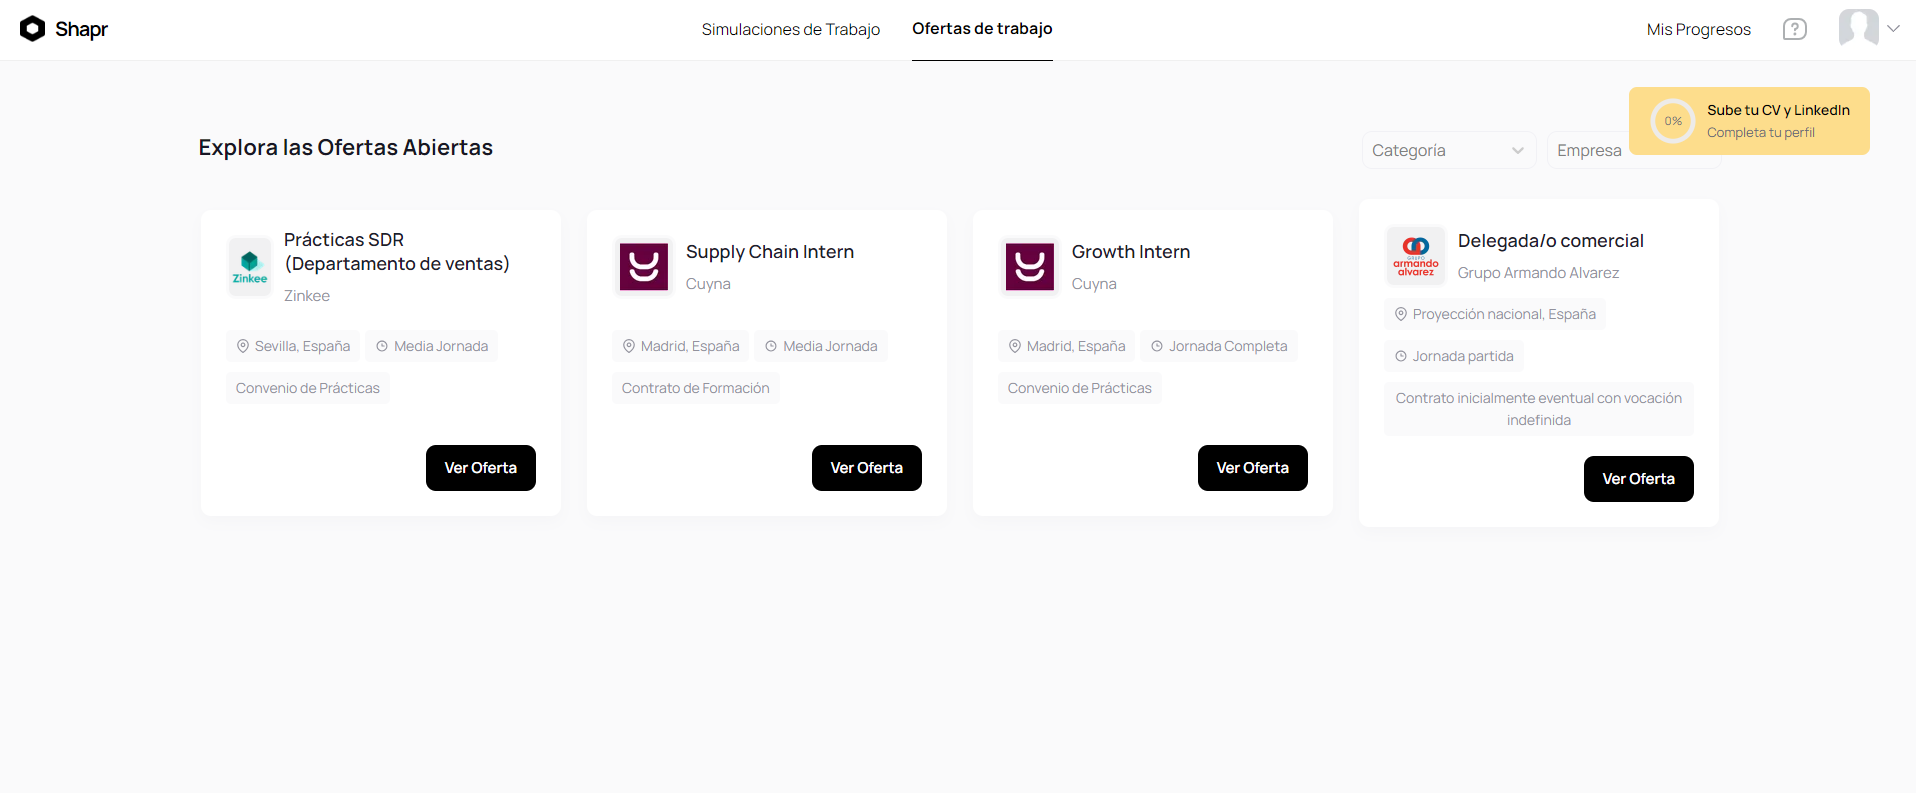
\includegraphics[width=0.95\textwidth]{figs/shapr-ofertas.png}
    \caption{Listado de ofertas laborales en Shapr ajustadas al perfil del usuario.}
    \label{fig:shapr-ofertas}
\end{figure}

% Conclusiones sobre aplicaciones basadas en coincidencias
\subsubsection{Conclusiones}

Las aplicaciones analizadas en este bloque comparten la idea de emparejamiento por
coincidencia, aunque con enfoques distintos. \textbf{Tinder} introduce la lógica del
\textit{interés mutuo} a partir de sugerencias generales, mientras que \textbf{Spotify}
aporta el concepto de \textbf{recomendación personalizada} y afinidad basada en
comportamientos previos.

\textbf{Shapr}, a diferencia de las anteriores, está orientada al ámbito profesional y
muestra ofertas adaptadas a la información del usuario, aunque sin usar competencias ni
mostrar un porcentaje de coincidencia. Su modelo sirve de inspiración por su
\textbf{presentación clara y filtrado automatizado}.

Estas soluciones aportan \textbf{ideas clave}, pero ninguna cubre el emparejamiento
profesional desde una perspectiva basada en competencias y afinidad técnica. Por ello, se
plantea la creación de una \textbf{plataforma específica} como la propuesta en este
\gls{tfg}.

% 2.2
\section{Evaluación de tecnologías}\label{sec:evaluacion-tecnologias}
% Análisis crítico de las tecnologías y sistemas de despliegue posibles y por qué se han seleccionado unas concretas.
